\documentclass[a4paper]{beamer}%handout


\usepackage{listings}
\usepackage{color}
 
\definecolor{codegreen}{rgb}{0,0.6,0}
\definecolor{codegray}{rgb}{0.5,0.5,0.5}
\definecolor{codepurple}{rgb}{0.58,0,0.82}
\definecolor{backcolour}{rgb}{0.95,0.95,0.92}


%% Add Matlab code
\usepackage{mcode}
%% Add Matlab code end


%% Add watermarks
%\usepackage{draftwatermark}
%% Add watermarks end
\usepackage[utf8]{inputenc}
\usepackage{multicol}
\usepackage{url}
\usepackage{hyperref}
\hypersetup{
	colorlinks=true,
	linkcolor=cyan,          % color of internal links (change box color with linkbordercolor)
    citecolor=green,        % color of links to bibliography
    filecolor=magenta,      % color of file links
    urlcolor=cyan           % color of external links
	}

\graphicspath{{img/}}

\mode<presentation> {

%\usetheme{default}%yes % use %\frametitle in all slides recommended
%\usetheme{AnnArbor}%no
%\usetheme{Antibes} %yes %favorite
%\usetheme{Bergen} %no
%\usetheme{Berkeley} %no
%\usetheme{Berlin} %no
%\usetheme{Boadilla} %yes % good use of paper space
%\usetheme{CambridgeUS} %yes %favorite %use %\frametitle recommended
%\usetheme{Copenhagen}%yes%noframetitle
%\usetheme{Darmstadt}%no
%\usetheme{Dresden}
%\usetheme{Frankfurt}
%\usetheme{Goettingen}
%\usetheme{Hannover}
%\usetheme{Ilmenau}%no
%\usetheme{JuanLesPins}
%\usetheme{Luebeck}
%\usetheme{Madrid}
%\usetheme{Malmoe}
%\usetheme{Marburg}
%\usetheme{Montpellier}
%\usetheme{PaloAlto}
%\usetheme{Pittsburgh}%no
%\usetheme{Rochester}%no
%\usetheme{Singapore}%yees
%\usetheme{Szeged}%no
%\usetheme{Warsaw}%no

% As well as themes, the Beamer class has a number of color themes
% for any slide theme. Uncomment each of these in turn to see how it
% changes the colors of your current slide theme.

%\usecolortheme{albatross}
%\usecolortheme{beaver}
%\usecolortheme{beetle}
%\usecolortheme{crane}
\usecolortheme{dolphin}
%\usecolortheme{dove}
%\usecolortheme{fly}
%\usecolortheme{lily}
%\usecolortheme{orchid}
%\usecolortheme{rose}
%\usecolortheme{seagull}
%\usecolortheme{seahorse}
%\usecolortheme{whale}
%\usecolortheme{wolverine}

\setbeamertemplate{footline} % To remove the footer line in all slides uncomment this line
%\setbeamertemplate{footline}[page number] % To replace the footer line in all slides with a simple slide count uncomment this line

\setbeamertemplate{navigation symbols}{} % To remove the navigation symbols from the bottom of all slides uncomment this line
}

%----------------------------------------------------------------------------------------
%	NEW COMMANDS
%----------------------------------------------------------------------------------------

\newcommand{\Conv}{\mathop{\scalebox{1.5}{\raisebox{-0.2ex}{$\ast$}}}}%
%\linespread{1.3}

%----------------------------------------------------------------------------------------
%	TITLE PAGE
%----------------------------------------------------------------------------------------

\title[Introduction]{Digital Image Processing} % The short title appears at the bottom of every slide, the full title is only on the title page

\author{Prof. Tiago Vieira} % Your name
\institute[UFAL] % Your institution as it will appear on the bottom of every slide, may be shorthand to save space
{
Universidade Federal de Alagoas \\ % Your institution for the title page
\medskip
\textit{tvieira@ic.ufal.br} % Your email address
}
\date{\today} % Date, can be changed to a custom date


%----------------------------------------------------------------------------------------
%	TITLE PAGE
%----------------------------------------------------------------------------------------

\subtitle{Fundamentals}

%------------------------------------------------

\begin{document}

%------------------------------------------------

\begin{frame}
\titlepage % Print the title page as the first slide
\end{frame}

%------------------------------------------------

\begin{frame}{Contents}
\setcounter{tocdepth}{1}
\tableofcontents
\end{frame}

%----------------------------------------------------------------------------------------
%	PRESENTATION SLIDES
%----------------------------------------------------------------------------------------

\section{Visual perception}

%----------------------------------------------------------------------------------------

\begin{frame}
The human eye.
\begin{columns}
\begin{column}{.3\textwidth}
\begin{itemize}
\item Diameter $\approx 20mm$.
\item Cornea/sclera; Choroid; Retina.
\end{itemize}
\end{column}
\begin{column}{.7\textwidth}
\begin{figure}
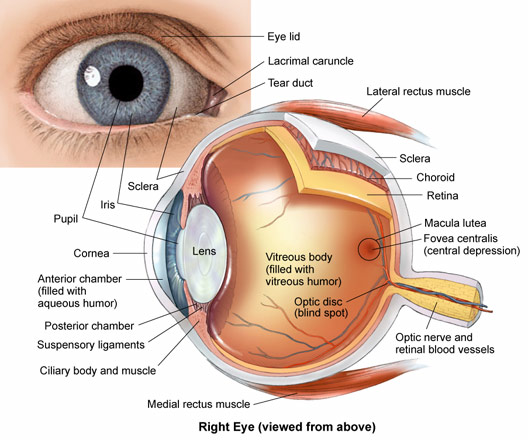
\includegraphics[width=\textwidth]{eye.jpg}
\end{figure}
\end{column}
\end{columns}
\end{frame}

%----------------------------------------------------------------------------------------

\begin{frame}
The human eye.
\begin{columns}
\begin{column}{.3\textwidth}
\begin{itemize}
\item Iris.
\item Pupil ($\phi\in [2,8] \text{mm}$).
\item Lens.
\end{itemize}
\end{column}
\begin{column}{.7\textwidth}
\begin{figure}
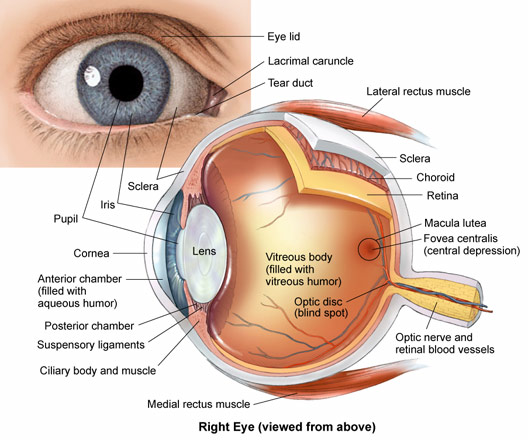
\includegraphics[width=\textwidth]{eye.jpg}
\end{figure}
\end{column}
\end{columns}
\end{frame}

%----------------------------------------------------------------------------------------

\begin{frame}
Retina.
\begin{itemize}
\item Innermost membrane of the eye.
\item Contains elements sensitive to light:
\end{itemize}
Light sensitiveness:
\begin{itemize}
\item Cones.
\begin{itemize}
\item $6-7$ million.
\item More densely distributed around the fovea ($\phi\approx 1.5$mm).
\item Highly sensitive to color.
\item Photopic vision (bright-light vision).
\end{itemize}
\end{itemize}
\end{frame}

%----------------------------------------------------------------------------------------

\begin{frame}
Light sensitiveness:
%\begin{columns}
%\begin{column}{.5\textwidth}
\begin{itemize}
\item Rods.
\begin{itemize}
\item $75-150$ million.
\item Scotopic vision (low level of illumination).
\item Give an overview of the Field-of-View (FOV).
\item Do not sense color.
\end{itemize}
\end{itemize}
%\end{column}
%\begin{column}{.6\textwidth}
\begin{figure}
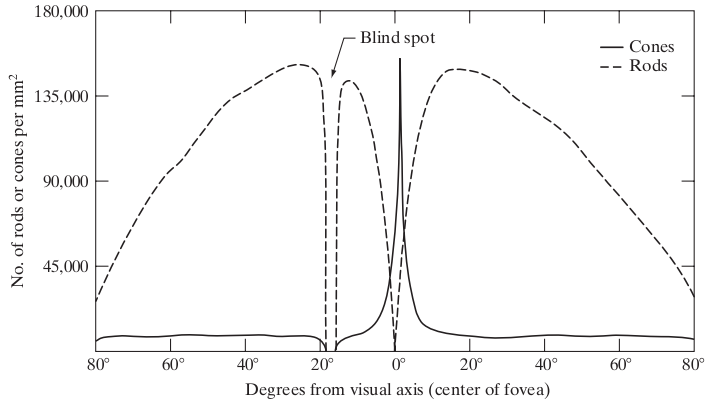
\includegraphics[width=.7\textwidth]{rodsAndConesDistro.png}
\end{figure}
%\end{column}
%\end{columns}
\end{frame}

%----------------------------------------------------------------------------------------

\begin{frame}
\begin{itemize}
\item Suppose that the fovea is a $1.5\times 1.5 mm^{2}$ square $\rightarrow$ and the density of cones $150k\text{ elem./mm}^{2}$. Then we have $\approx 337k$ elements.
\item A medium resolution CCD chip no larger than $5\text{ mm}\times\text{5 mm}$ has this amount of elements.
\end{itemize}
\begin{block}{}
Current electronic imaging sensors are comparable to the eye's resolution.
\end{block}
\end{frame}

%----------------------------------------------------------------------------------------

\begin{frame}
The lens:
\begin{itemize}
\item Fixed w.r.t. the retina ($\approx 17\text{ mm}$).
\item Range of focal length $\approx [14,17]$ mm.
\item $h=17\cdot 15/100	= 2.55$ mm.
\end{itemize}
\begin{figure}
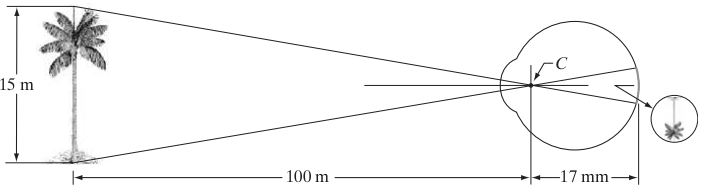
\includegraphics[width=.9\textwidth]{eyeGeometry.png}
\end{figure}
\end{frame}

\begin{frame}
The lens:
\begin{itemize}
\item The retinal image is focused primarily on the fovea.
\item Perception senses the relative excitation of light receptors.
\item Light is converted into electric signals, interpreted by the brain.
\end{itemize}
\begin{figure}
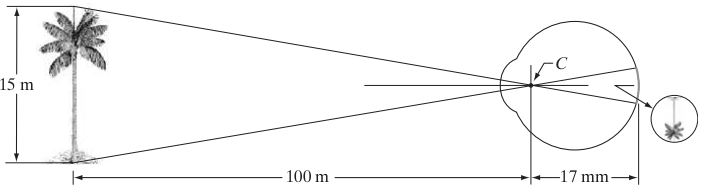
\includegraphics[width=.9\textwidth]{eyeGeometry.png}
\end{figure}
\end{frame}

%----------------------------------------------------------------------------------------

\subsection{Brightness adaptation and discrimination}

\begin{frame}
Brightness adaptation and discrimination:
\begin{columns}
\begin{column}{.5\textwidth}
\begin{itemize}
\item The eye can adapt to a huge amount of intensity levels ($\backsim 10^{10}$).
\item Subjective brightness is a logarithmic function  of the light intensity incident in the human eye.
\end{itemize}
\end{column}
\begin{column}{.5\textwidth}
\begin{figure}
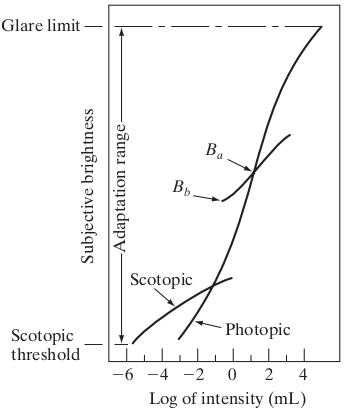
\includegraphics[width=\textwidth]{subjectiveBrightness.png}
\end{figure}
\end{column}
\end{columns}
\end{frame}

%----------------------------------------------------------------------------------------

\begin{frame}
Eye ability to discriminate between \textit{changes} in illumination intensities.
\begin{itemize}
\item Weber ratio = $\Delta I_{c}/I$.
\end{itemize}
\begin{columns}
\begin{column}{.5\textwidth}
\begin{figure}
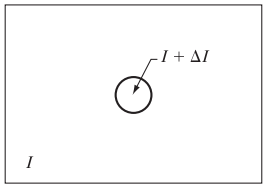
\includegraphics[width=.8\textwidth]{brightnessDiscrimination.png}
\end{figure}
\end{column}
\begin{column}{.5\textwidth}
\begin{figure}
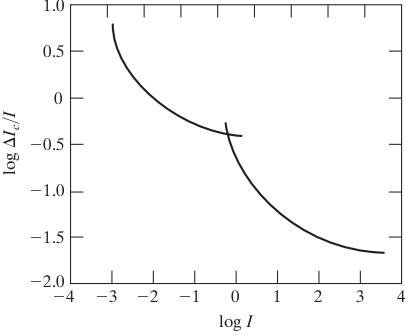
\includegraphics[width=\textwidth]{webersCurves.png}
\end{figure}
\end{column}
\end{columns}
\end{frame}

%----------------------------------------------------------------------------------------

\begin{frame}
Perceived brightness is not a simple function of intensity (Mach bands).
\begin{figure}
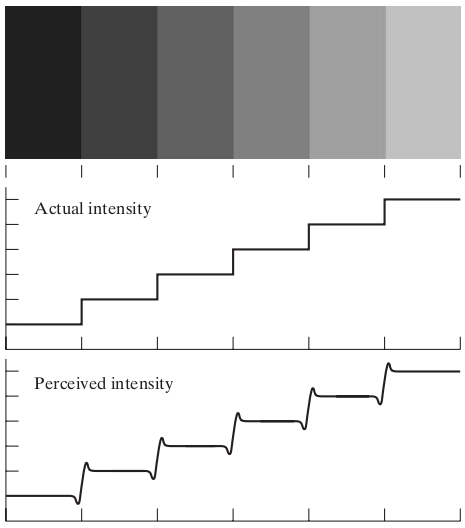
\includegraphics[width=.5\textwidth]{machBand.png}
\end{figure}
\end{frame}

%----------------------------------------------------------------------------------------

\begin{frame}
Perceived brightness is not a simple function of intensity (Simultaneous contrast).
\begin{figure}

\includegraphics[width=.8\textwidth]{simultaneousContrast.png}
\end{figure}
\end{frame}

%----------------------------------------------------------------------------------------

\begin{frame}
Optical illusions:
\begin{figure}
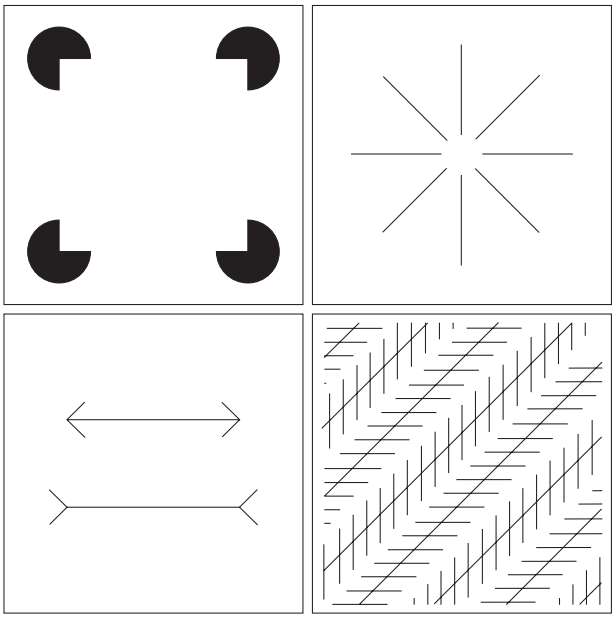
\includegraphics[width=.6\textwidth]{opticalIllusion1.png}
\end{figure}
\end{frame}

%----------------------------------------------------------------------------------------

\section{Light}

%----------------------------------------------------------------------------------------

\begin{frame}
\frametitle{Light}
Electromagnetic radiation can be expressed in terms of wavelength ($\lambda$), frequency ($\nu$) or energy ($E$).
\begin{equation}
c=\lambda\nu
\end{equation}
\begin{equation}
E=h\nu
\end{equation}
Where $c\approx 3\cdot 10^{8}\text{ m/s}$ is the speed of light and $h=6.62\cdot 10^{-34}m^{2}kg/s$ is the Plank constant.
\begin{figure}
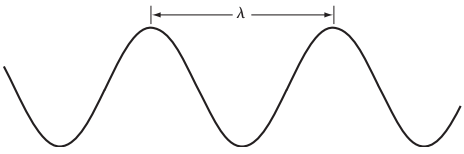
\includegraphics[width=.5\textwidth]{wave.png}
\end{figure}
\end{frame}

%----------------------------------------------------------------------------------------

\begin{frame}
\begin{itemize}
\item If a sensor can be developed that is capable of detecting energy radiated by a band of the electromagnetic spectrum, we can image events of interest in that band.
\item Example: water molecule ($\approx 10^{-10}m)$. We need a source emitting in the far ultraviolet or soft X-ray region.
\item Remember that other sources can be used for imaging, such as sound, electron microscopy and synthetic images.
\end{itemize}
\end{frame}

%----------------------------------------------------------------------------------------

\section{Image sensing and acquisition}

%----------------------------------------------------------------------------------------

\begin{frame}
\begin{enumerate}
%\item Illumination and scene - a general concept.
\item Sensor arrangements:
\end{enumerate}
\begin{columns}
\begin{column}{.7\textwidth}
\begin{figure}
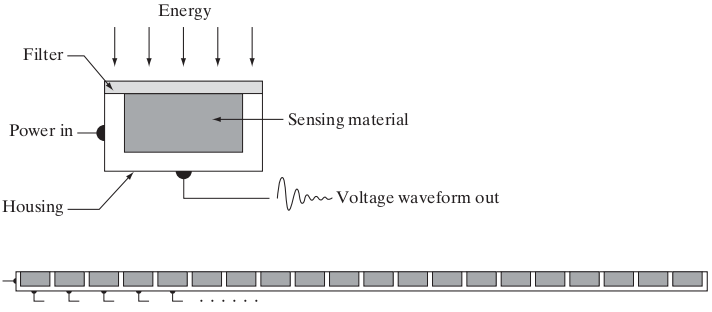
\includegraphics[width=\textwidth]{singleImagingSensor.png}
\end{figure}
\end{column}
\begin{column}{.3\textwidth}
\begin{figure}
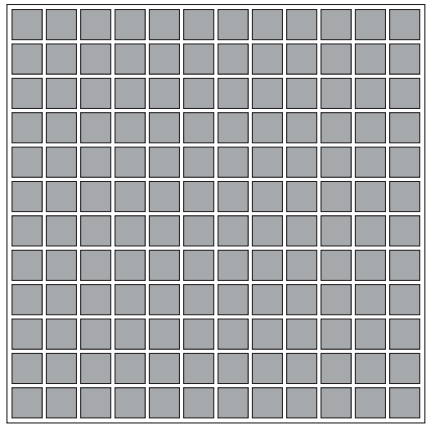
\includegraphics[width=\textwidth]{2dImagingSensor.png}
\end{figure}
\end{column}
\end{columns}
\end{frame}

%----------------------------------------------------------------------------------------

\subsection{Single sensor}

%----------------------------------------------------------------------------------------

\begin{frame}
Image acquisition with single sensor.
\begin{itemize}
\item Photo-diode.
\item Displacement is necessary to generate 2D images.
\item \textit{Microdensiometers}.
\item Laser with moving mirrors.
\end{itemize}
\begin{figure}
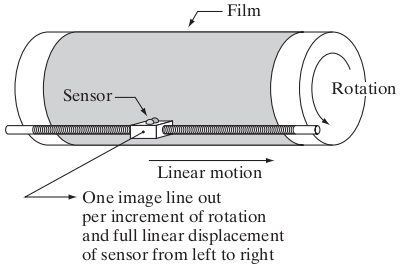
\includegraphics[width=.5\textwidth]{singleSensorPlusMotion.png}
\end{figure}
\end{frame}

%----------------------------------------------------------------------------------------

\subsection{Sensor strips}

%----------------------------------------------------------------------------------------

\begin{frame}
Image acquisition using sensor strips.
\begin{itemize}
\item Airborne imaging applications.
\item Comp. Axial Tomography (CAT) scan.
\end{itemize}
\begin{figure}
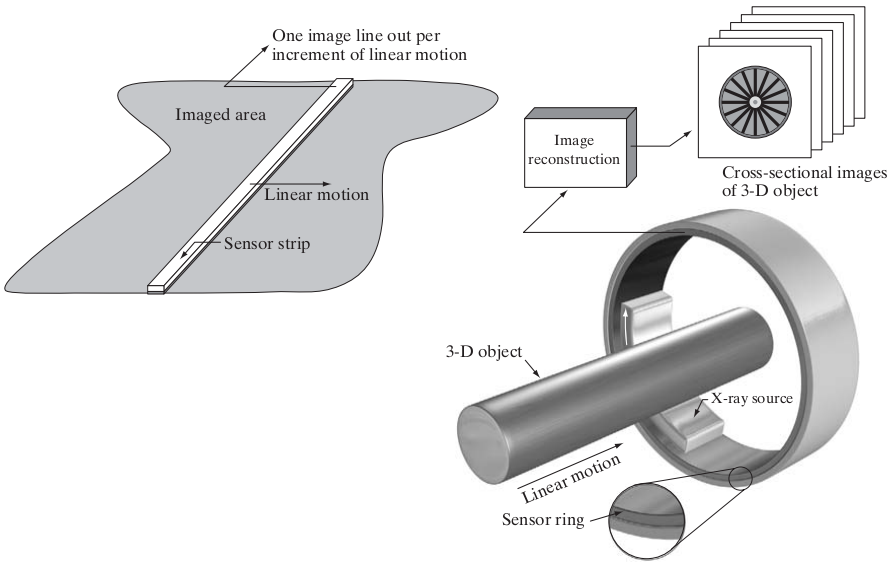
\includegraphics[width=.8\textwidth]{sensorStrip.png}
\end{figure}
\end{frame}

%----------------------------------------------------------------------------------------

\subsection{Sensor arrays}

%----------------------------------------------------------------------------------------

\begin{frame}
Sensor arrays.
\begin{itemize}
\item No motion necessary.
\item Typical in cameras.
\item $4k \times 4k = 16$~Mpx.
\end{itemize}
\begin{figure}
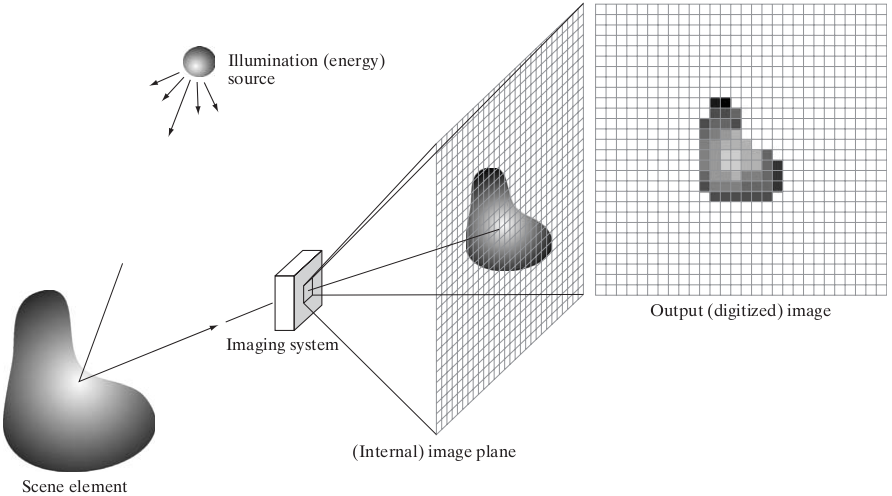
\includegraphics[width=.8\textwidth]{sensorArray.png}
\end{figure}
\end{frame}

%----------------------------------------------------------------------------------------

\begin{frame}
Sensor arrays.
\begin{figure}
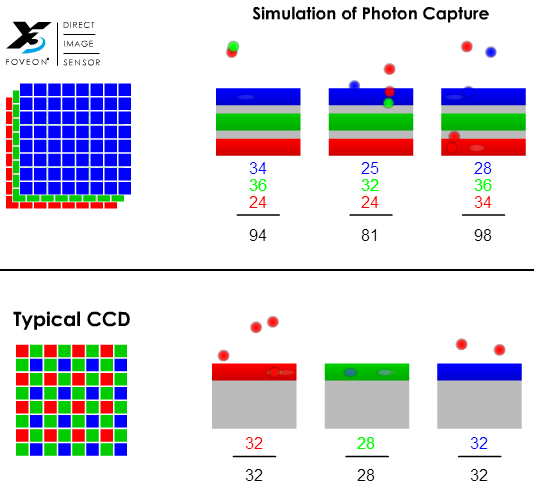
\includegraphics[width=.6\textwidth]{foveon-1.png}
\end{figure}
\end{frame}

%----------------------------------------------------------------------------------------

\begin{frame}
Sensor arrays.
\begin{figure}
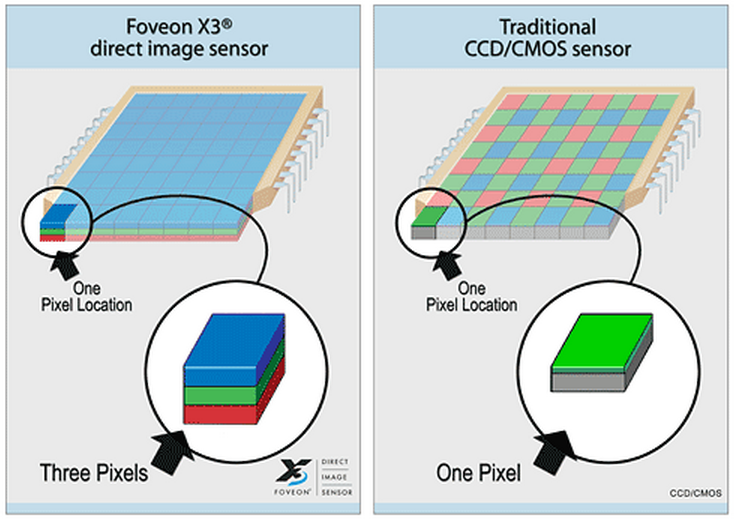
\includegraphics[width=.6\textwidth]{foveon-2.png}
\end{figure}
\end{frame}

%----------------------------------------------------------------------------------------

\begin{frame}
Sensor arrays.
\begin{figure}
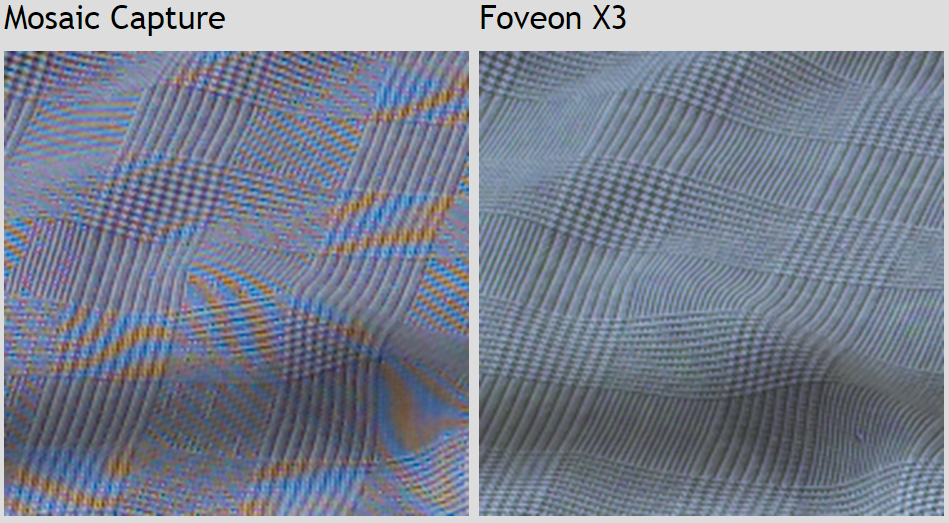
\includegraphics[width=\textwidth]{foveon-3.png}
\end{figure}
\end{frame}

%----------------------------------------------------------------------------------------

\subsection{Image formation model}

%----------------------------------------------------------------------------------------

\begin{frame}
Image formation model:
\begin{itemize}
\item $0\leq f(x,y)<\infty$, image. Determined by the product between:
\begin{itemize}
\item $i(x,y)$, illumination, determined by the light source ($0\leq i(x,y)<\infty$).
\item $r(x,y)$, reflectance, determined by object's characteristics ($0\leq r(x,y)\leq 1$).
\end{itemize}
\begin{equation}
f(x,y) = i(x,y) \times r(x,y)
\end{equation}
\end{itemize}
\end{frame}

%----------------------------------------------------------------------------------------

\begin{frame}
\begin{itemize}
\item $I$, intensity level, value of the image at $(x,y)$.
\item $L_{min} \leq l \leq L_{max}$, interval, gray scale.
\item Typically, the gray scale is shifted to $[0,L-1]$, where $l=0$ is black and $l=L-1$ means white.
\item Typically, $L=2^{k}$. For \texttt{uint8} image format, $k=8$ bits and there are $256$ levels.
\end{itemize}
\end{frame}

%----------------------------------------------------------------------------------------

\section{Image sampling and quantization}

%----------------------------------------------------------------------------------------

\subsection{Basic concepts of sampling}

%----------------------------------------------------------------------------------------

\begin{frame}
Generation of digital images from sampled data.
\begin{itemize}
\item Sampling.
\item Quantization.
\end{itemize}
\begin{figure}
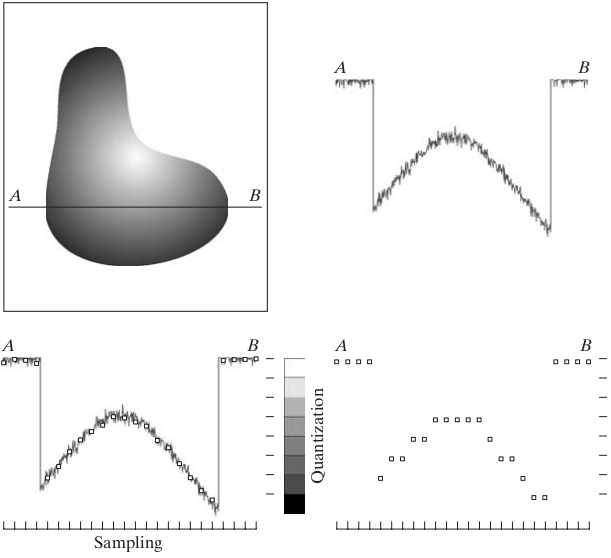
\includegraphics[width=.6\textwidth]{samplingAndQuantization.png}
\end{figure}
\end{frame}

%----------------------------------------------------------------------------------------

\begin{frame}
\begin{figure}
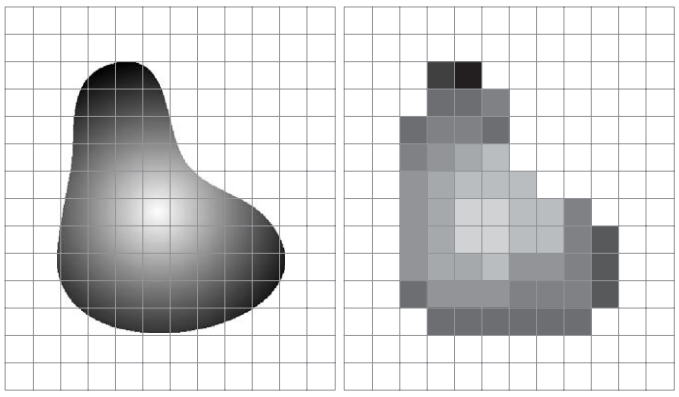
\includegraphics[width=.7\textwidth]{sampledPear.png}
\end{figure}
\end{frame}

%----------------------------------------------------------------------------------------

\subsection{Image representation}

%----------------------------------------------------------------------------------------

\begin{frame}
Spatial domain:
\begin{itemize}
\item Spatial coordinates $(x,y)$ are different from sensor coordinates $(u,v)$.
\item $x=0,\ldots,M-1$.
\item $y=0,\ldots,N-1$.
\end{itemize}
\begin{columns}
\begin{column}{.4\textwidth}
\begin{figure}
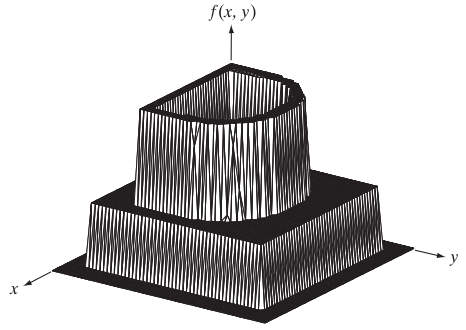
\includegraphics[width=\textwidth]{imageRepresentation-1.png}
\end{figure}
\end{column}
\begin{column}{.6\textwidth}
\begin{figure}
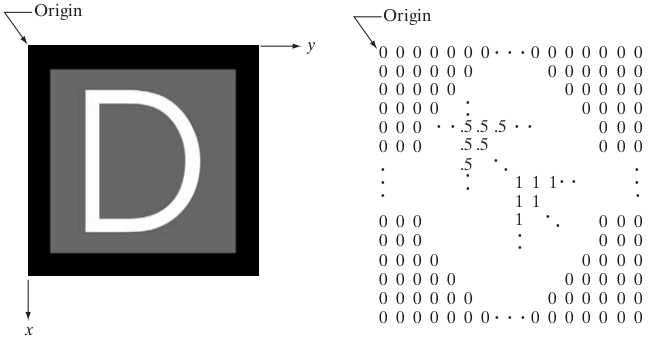
\includegraphics[width=\textwidth]{imageRepresentation-2.png}
\end{figure}
\end{column}
\end{columns}
\end{frame}

%----------------------------------------------------------------------------------------

\begin{frame}
An image is an $M\times N$ matrix, where each cell contains an intensity.
\begin{figure}
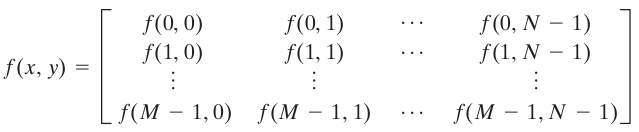
\includegraphics[width=.7\textwidth]{eq_f_x_y.png}
\end{figure}
\end{frame}

%----------------------------------------------------------------------------------------

\subsection{Spatial and intensity resolution}

%----------------------------------------------------------------------------------------

\begin{frame}
Consider a chart:
\begin{figure}

\includegraphics[width=.3\textwidth]{prison.png}
\end{figure}
Image resolution is the largest number of \textit{discernible} line pairs per unit distance (dots per inch -- \textit{dpi}).
\begin{itemize}
\item Newspapers (75 dpi).
\item Magazines (133 dpi).
\item Glossy brochures (175 dpi).
\end{itemize}
\end{frame}

%----------------------------------------------------------------------------------------

\begin{frame}
\begin{itemize}
\item An image with $1024\times 1024$ resolution has how many dpi?
\item One must state the spatial dimension encompassed by the image.
\end{itemize}
\end{frame}

%----------------------------------------------------------------------------------------

\begin{frame}
\begin{columns}
\begin{column}{.5\textwidth}
\begin{figure}
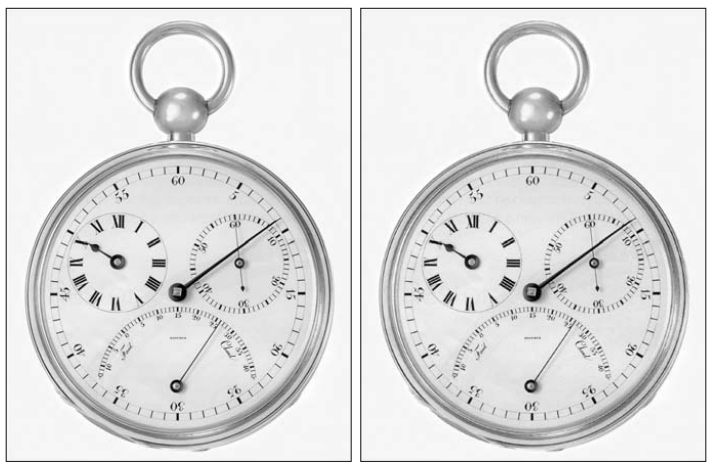
\includegraphics[width=\textwidth]{watches-1.png}
\end{figure}
\end{column}
\begin{column}{.5\textwidth}
\begin{figure}
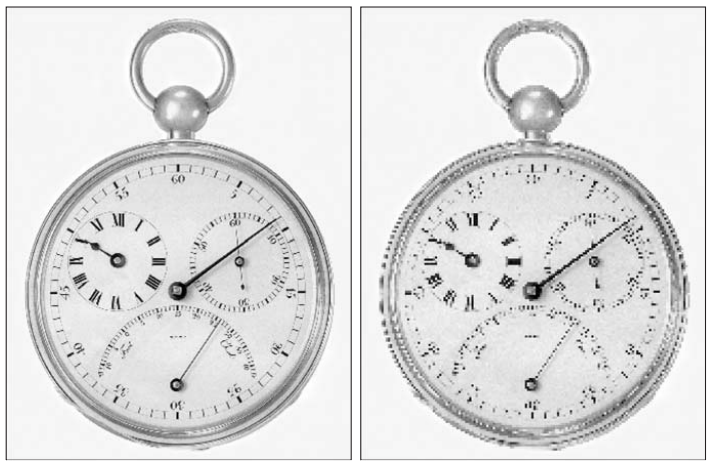
\includegraphics[width=\textwidth]{watches-2.png}
\end{figure}
\end{column}
\end{columns}
\end{frame}

%----------------------------------------------------------------------------------------

\begin{frame}
\begin{block}{Intensity resolution}
Smallest discernible change in intensity level.
\end{block}
\end{frame}

%----------------------------------------------------------------------------------------

\begin{frame}
Number of intensity levels: 256, 128, 64, 32, 16, 8, 4, 2. Observe the \textit{false contouring}.
\begin{columns}
\begin{column}{.5\textwidth}
\begin{figure}
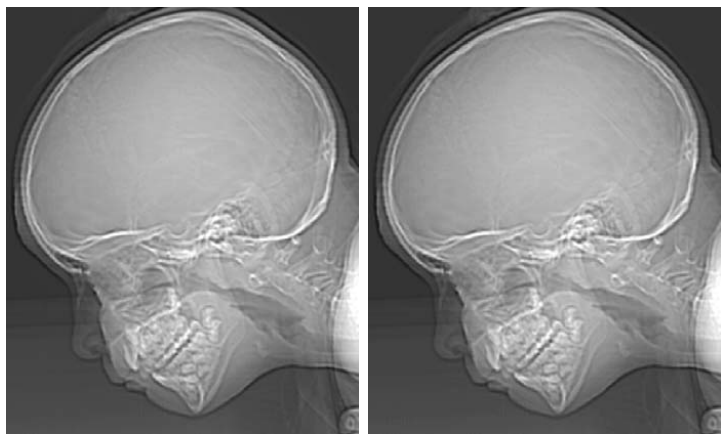
\includegraphics[width=\textwidth]{skull-1.png}
\end{figure}
\end{column}
\begin{column}{.5\textwidth}
\begin{figure}
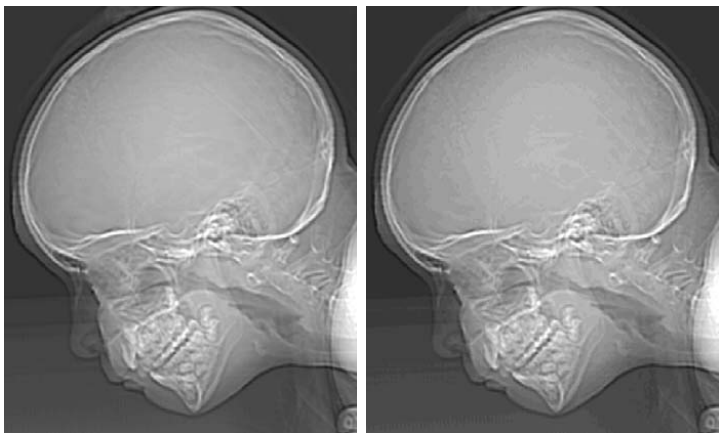
\includegraphics[width=\textwidth]{skull-2.png}
\end{figure}
\end{column}
\end{columns}
\begin{columns}
\begin{column}{.5\textwidth}
\begin{figure}
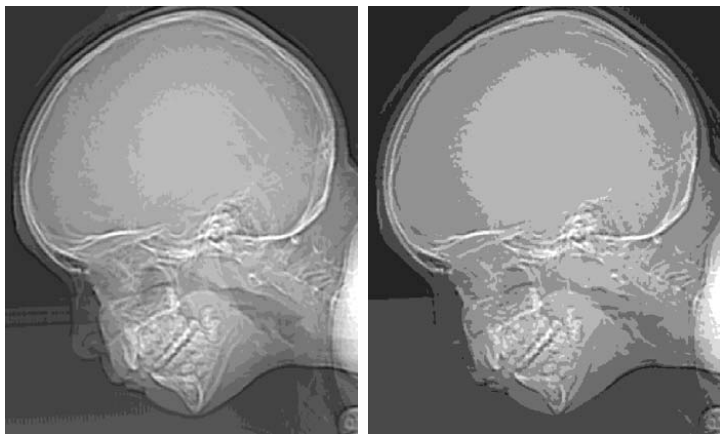
\includegraphics[width=\textwidth]{skull-3.png}
\end{figure}
\end{column}
\begin{column}{.5\textwidth}
\begin{figure}
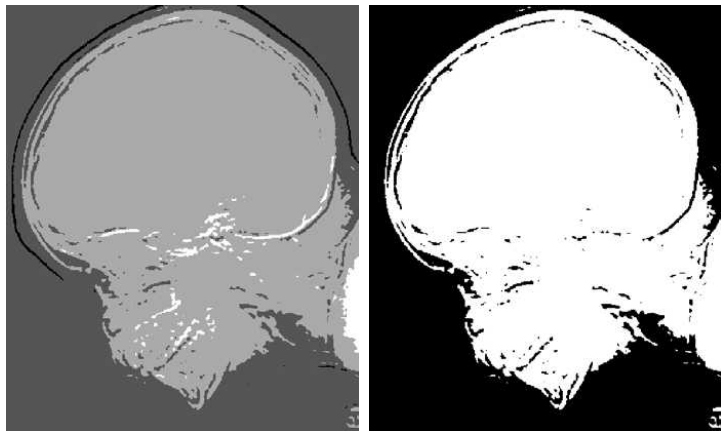
\includegraphics[width=\textwidth]{skull-4.png}
\end{figure}
\end{column}
\end{columns}
\end{frame}

%----------------------------------------------------------------------------------------

\begin{frame}
Concept of image quality is subjective. Where $N$ is dimension and $2^k$ gray levels.
\begin{itemize}
\item Isopreference curves in the $Nk$-plane.
\item Tend to be more vertical as the detail in the image increases.
\item I. e., the more detail, the less the intensity levels needed.
\end{itemize}
\begin{columns}
\begin{column}{.7\textwidth}
\begin{figure}
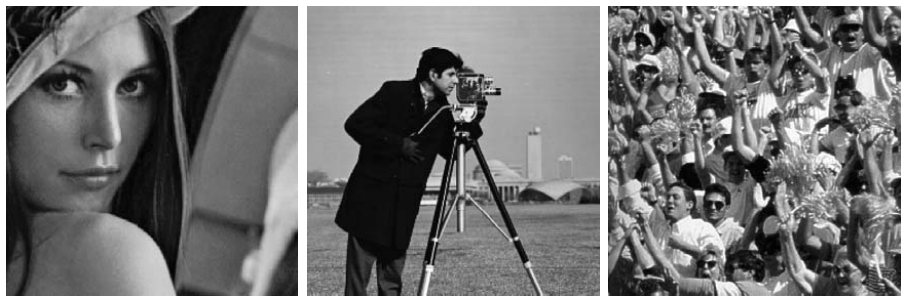
\includegraphics[width=\textwidth]{isocurves-1.png}
\end{figure}
\end{column}
\begin{column}{.3\textwidth}
\begin{figure}
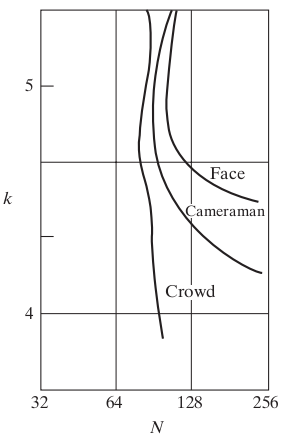
\includegraphics[width=.7\textwidth]{isocurves-2.png}
\end{figure}
\end{column}
\end{columns}
\end{frame}

%----------------------------------------------------------------------------------------

\begin{frame}
\begin{block}{Rough rule of thumb}
Images of size $256\times 256$ pixels with $64$ intensity levels and printed on a size format on the order of $5\times 5$~cm are about the lowest spatial and intensity resolution images that can be expected to be reasonably free of objectionable sampling checkerboards and false contouring.
\end{block}
\end{frame}

%----------------------------------------------------------------------------------------

\subsection{Image interpolation}

%----------------------------------------------------------------------------------------

\begin{frame}
\frametitle{Interpolation}
Often used in:
\begin{itemize}
\item Zooming.
\item Shrinking.
\item Rotating.
\item Geometric corrections.
\end{itemize}
\end{frame}

%----------------------------------------------------------------------------------------

\begin{frame}
Interpolation methods:
\begin{itemize}
\item Nearest-neighbor.
\begin{itemize}
\item Simple but introduces artifacts.
\end{itemize}
\item Bilinear interpolation - New point between 4 points (coefficients).
\begin{equation}
v(x,y) = ax + by + cxy + d.
\end{equation}
\item Bicubic interpolation (standard, used in \textit{Photoshop}) - 16 coefficients.
\begin{equation}
v(x,y) = \sum_{i=0}^{3}\sum_{j=0}^{3}a_{ij}x^{i}y^{j}.
\end{equation}
\end{itemize}
\end{frame}

%----------------------------------------------------------------------------------------

\begin{frame}
\begin{figure}
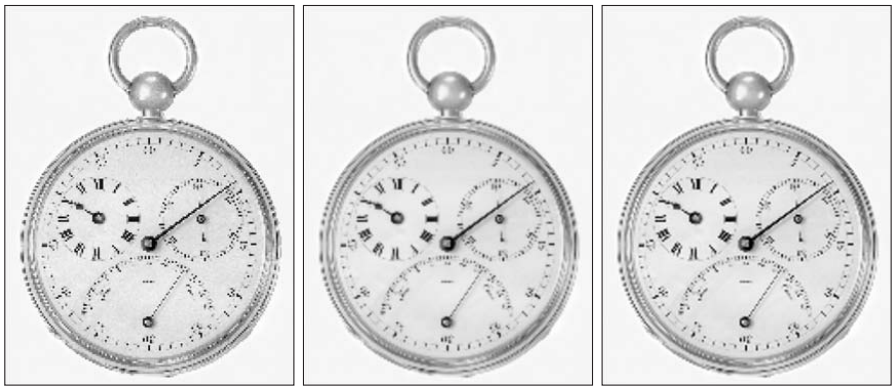
\includegraphics[width=.6\textwidth]{interpolationWatches-1.png}
\end{figure}
\begin{figure}
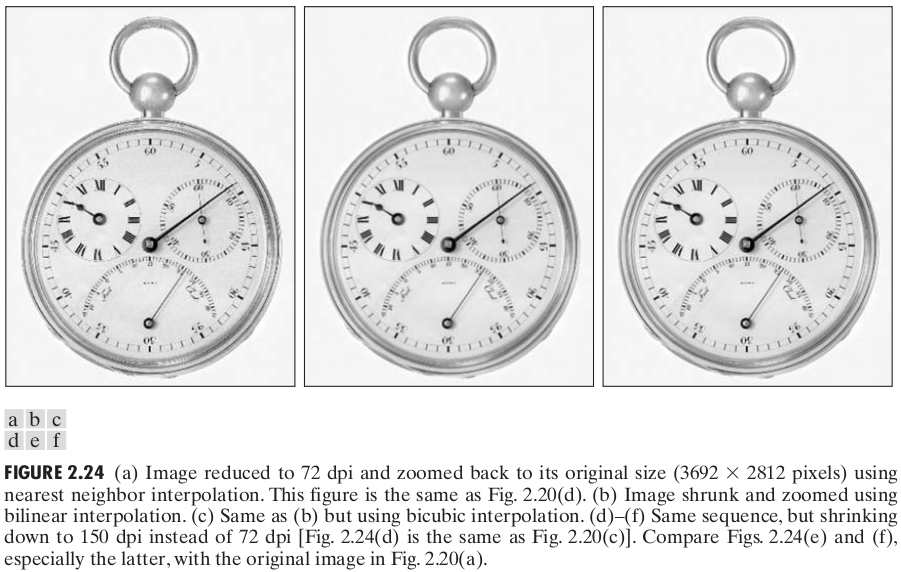
\includegraphics[width=.6\textwidth]{interpolationWatches-2.png}
\end{figure}
\end{frame}

%----------------------------------------------------------------------------------------

\section{Basic relationships between pixels}

%----------------------------------------------------------------------------------------

\subsection{Neighbors of a pixel}

%----------------------------------------------------------------------------------------

\begin{frame}
\frametitle{Basic relationships between pixels}
\begin{itemize}
\item $N_{4}(p)$ - the set of 4-\textit{neighbors} of pixel $p$ have coordinates \[(x+1,y),(x-1,y),(x,y+1),(x,y-1).\]
\item $N_{D}(p)$ - the set of 4-\textit{diagonal neighbors} of pixel $p$ whose coordinates are \[(x+1,y+1),(x-1,y-1),(x+1,y-1),(x-1,y+1).\]
\item $N_{8}(p) = N_{4}(p) \cup N_{D}(p)$.
\item Neighbor coordinates may fall outside the image range.
\end{itemize}
\end{frame}

%----------------------------------------------------------------------------------------

\subsection{Adjacency, Connectivity, Regions and Boundaries}

%----------------------------------------------------------------------------------------

\begin{frame}
Let $V$ be the set of values defining adjacency (Binary image, $V={1}$).
\begin{itemize}
\item 4-\textit{adjacency}. Two pixels $p$ and $q$ with values from $V$ are 4-adjacent if $q \in N_{4}(p)$.
\item 8-\textit{adjacency}. Two pixels $p$ and $q$ with values from $V$ are 8-adjacent if $q \in N_{8}(p)$.
\end{itemize}
\end{frame}

%----------------------------------------------------------------------------------------

\begin{frame}
Let $V$ be the set of values defining adjacency (Binary image, $V={1}$).
\begin{itemize}
\item m-\textit{adjacency} (mixed adjacency). Two pixels $p$ and $q$ with values from $V$ are
m-adjacent if
\begin{itemize}
\item $q\in N_{4}(p)$, or
\item $q\in N_{D}(p)$ \textit{and} the set $N_{4}(p) \cap N_{4}(q)$ has no pixels whose values are from $V$.
\end{itemize}
\end{itemize}
\begin{figure}
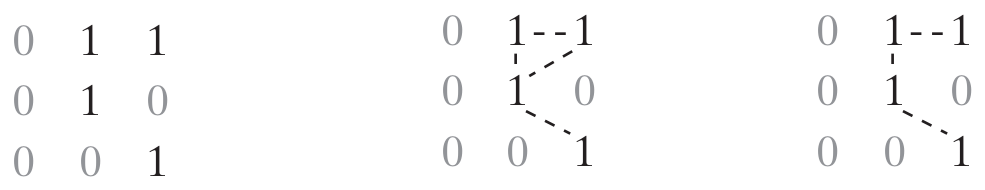
\includegraphics[width=.8\textwidth]{adjacency-1.png}
\end{figure}
\end{frame}

%----------------------------------------------------------------------------------------

\begin{frame}
Mixed adjacency is a modification of 8-adjacency. It is introduced to eliminate the ambiguities that often arise when 8-adjacency is used.
\end{frame}

%----------------------------------------------------------------------------------------

\begin{frame}
A (digital) path (or curve) from pixel $p$ with coordinates $(x,y)$ to pixel $q$ with coordinates $(s,t)$ is a sequence of distinct pixels with coordinates
\[
(x_{0},y_{0}),(x_{1},y_{1}),\ldots ,(x_{n},y_{n})
\]
where:
\begin{itemize}
\item $(x_{0},y_{0}) = (x,y)$.
\item $(x_{n},y_{n}) = (s,t)$.
\item And pixels $(x_{i}, y_{i})$ and $(x_{i-1}, y_{i-1})$ are adjacent for $1\leq i \leq n$.
\item $n = $ length of the path.
\end{itemize}
If $(x_{0},y_{0}) = (x_{n},y_{n})$ the path is closed.
Paths are defined as 4-, 8-, or \textit{m}- paths.
\end{frame}

%----------------------------------------------------------------------------------------

\begin{frame}
Let $S$ represent a subset of pixels in an image.
\begin{itemize}
\item Two pixels \textit{p} and \textit{q} are said to be connected in $S$ if there exists a path between them consisting entirely of pixels in $S$.
\item For any pixel $p$ in $S$, the set of pixels that are connected to it in $S$ is
called a connected component of $S$.
\item If it only has one connected component, then set $S$ is called a connected set.
\end{itemize}
\end{frame}

%----------------------------------------------------------------------------------------

\begin{frame}
\begin{block}{Connected set}
A subset $R$ of pixels in an image is called a \textit{region} of the image if $R$ is a connected set.
\end{block}
Two regions $R_{i}$ and $R_{j}$ are said to be adjacent if their union forms a connected set.
\begin{figure}
\centering
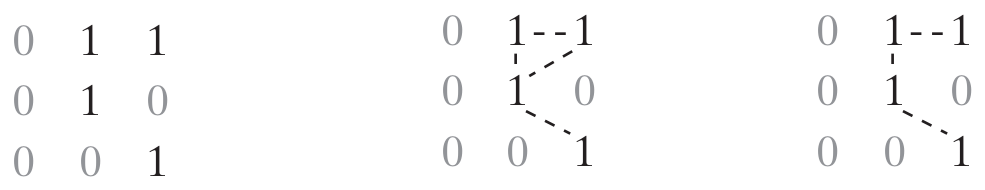
\includegraphics[width=.4\textwidth]{adjacency-1.png}
\end{figure}
\begin{figure}
\centering
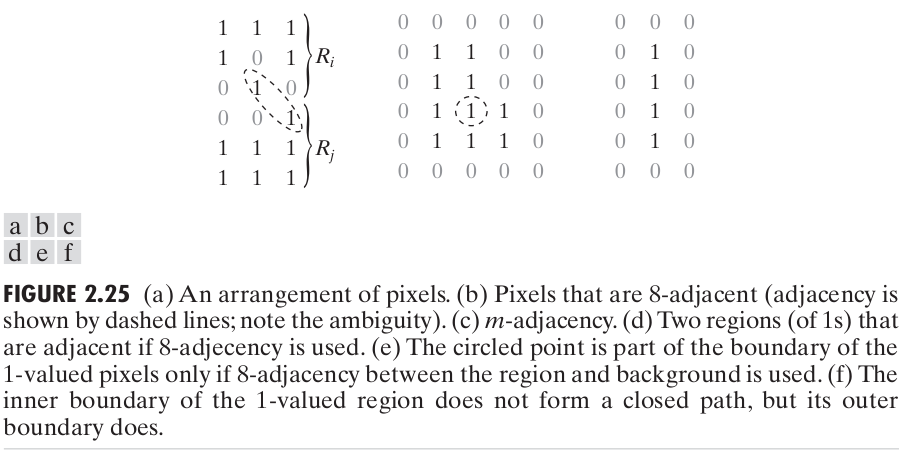
\includegraphics[width=.7\textwidth]{adjacency-2.png}
\end{figure}
\end{frame}

%----------------------------------------------------------------------------------------

\begin{frame}
\begin{block}{Boundary}
The boundary (border or contour) of a region $R$ is the set of pixels that have at least one background neighbor.
\end{block}
\end{frame}

%----------------------------------------------------------------------------------------

\subsection{Distance Measures}

%----------------------------------------------------------------------------------------

\begin{frame}
For pixels $p$, $q$ and $z$, with respective coordinates $(x, y)$, $(s, t)$, and $(v, w)$, $D$
is a distance function or metric if
\begin{itemize}
\item $D(p,q) \geq 0$ ($D(p,q) = 0$ if $p=q$).
\item $D(p,q) = D(q,p)$, and
\item $D(p,z) < D(p,q) + D(q,z)$.
\end{itemize}
The Euclidean distance between $p$ and $q$ is defined as
\[
D_{e}(p,q) = \left [ (x-s)^{2} + (y-t)^{2} \right ]^{1/2}.
\]
\end{frame}

%----------------------------------------------------------------------------------------

\begin{frame}
Other distances:
\begin{columns}
\begin{column}{.5\textwidth}
\begin{itemize}
\item City-block distance
\[
D_{4}(p,q) = |x-s| + |y-t|.
\]
\end{itemize}
\begin{figure}
\centering
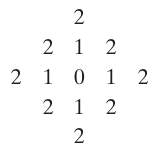
\includegraphics[width=.6\textwidth]{distance-1.png}
\end{figure}
\end{column}
\begin{column}{.5\textwidth}
\begin{itemize}
\item The $D_{8}$ distance
\[
D_{8}(p,q) = \text{max}(|x-s|,|y-t|).
\]
\end{itemize}
\begin{figure}
\centering
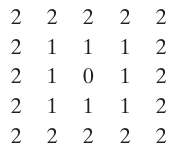
\includegraphics[width=.6\textwidth]{distance-2.png}
\end{figure}
\end{column}
\end{columns}
\end{frame}

%----------------------------------------------------------------------------------------


\begin{frame}
\begin{itemize}
\item $D_{4}$ and $D_{8}$ distances involve only coordinates of the points.
\item $D_{m}$ (\textit{m}-adjacency)) distance between 2 points = shortest \textit{m}-path between the points.
\item Now the pixels in between matter.
\end{itemize}
\begin{table}
\centering
\begin{tabular}{|c|c|c|}
\hline 
 & $p_3$ & $p_4$ \\ 
\hline 
$p_1$ & $p_2$ &  \\ 
\hline 
$p$ &   &   \\ 
\hline 
\end{tabular}
\end{table}
\begin{columns}
\begin{column}{.3\textwidth}
\begin{table}
\centering
\begin{tabular}{|c|c|c|}
\hline 
 & 0 & 1 \\ 
\hline 
0 & 1 &  \\ 
\hline 
1 &   &   \\ 
\hline 
\end{tabular}
\end{table}
\[pp_{2}p_{4}\]
\end{column}
\begin{column}{.3\textwidth}
\begin{table}
\centering
\begin{tabular}{|c|c|c|}
\hline 
 & 0 & 1 \\ 
\hline 
1 & 1 &  \\ 
\hline 
1 &   &   \\ 
\hline 
\end{tabular}
\end{table}
\[pp_{1}p_{2}p_{4}\]
\end{column}
\begin{column}{.3\textwidth}
\begin{table}
\centering
\begin{tabular}{|c|c|c|}
\hline 
 & 1 & 1 \\ 
\hline 
1 & 1 &  \\ 
\hline 
1 &   &   \\ 
\hline 
\end{tabular}
\end{table}
\[pp_{1}p_{2}p_{3}p_{4}\]
\end{column}
\end{columns}
\end{frame}

%----------------------------------------------------------------------------------------

\section{Mathematical tools}

%----------------------------------------------------------------------------------------

\subsection{Array vs Matrix operations}

%----------------------------------------------------------------------------------------

\begin{frame}
\frametitle{Mathematical Tools}
Attention:
\begin{itemize}
\item Array operation is made pixel-by-pixel.
\item Matrix operations are carried out using matrix theory.
\item Henceforth assume array operation unless stated otherwise.
\end{itemize}
\begin{figure}
\centering
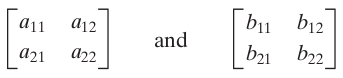
\includegraphics[width=.4\textwidth]{array-1.png}
\end{figure}
\end{frame}

%----------------------------------------------------------------------------------------

\begin{frame}
Array product:
\begin{figure}
\centering
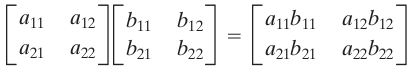
\includegraphics[width=.5\textwidth]{array-2.png}
\end{figure}
Matrix product:
\begin{figure}
\centering
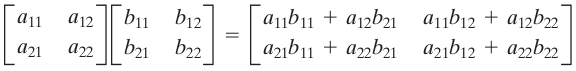
\includegraphics[width=.7\textwidth]{array-3.png}
\end{figure}
\end{frame}

%----------------------------------------------------------------------------------------

\subsection{Linear versus Nonlinear operations}

%----------------------------------------------------------------------------------------

\begin{frame}
Linear versus Nonlinear operations:
\begin{itemize}
\item Consider a general operator, $H$, that produces an output image, $g(x, y)$, for a given input image, $f(x, y)$:
\begin{equation}
H[f(x,y)]=g(x,y).
\end{equation}
\item $H$ is linear if
\begin{equation}
H[a_{i}f_{i}(x,y) + a_{j}f_{j}(x,y)] = a_{i}H[f_{i}(x,y)] + a_{j} H[f_{j}(x,y)].
\end{equation}
\item Where $a_{i}, a_{j}, f_{i}(x,y)$ and $f_{j}(x,y)$ are arbitrary constants and images (of the same size).
\end{itemize}
\end{frame}

%----------------------------------------------------------------------------------------

\begin{frame}
\begin{itemize}
\item Linear example: The sum operator ($\sum$):
\begin{figure}
\centering
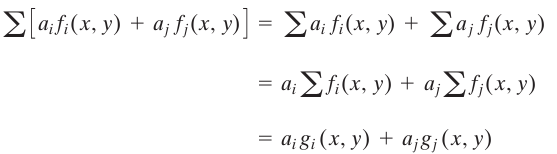
\includegraphics[width=.8\textwidth]{sum-operator.png}
\end{figure}
\end{itemize}
\end{frame}

%----------------------------------------------------------------------------------------

\begin{frame}
\begin{columns}
\begin{column}{.5\textwidth}
\begin{figure}
\centering
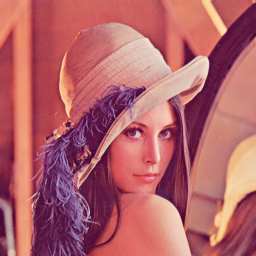
\includegraphics[width=\textwidth]{linear-1.png}
\end{figure}
\end{column}
\begin{column}{.5\textwidth}
\begin{figure}
\centering
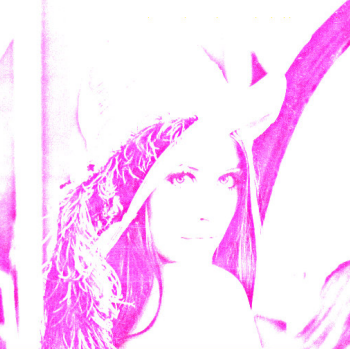
\includegraphics[width=\textwidth]{linear-2.png}
\end{figure}
\end{column}
\end{columns}
\end{frame}

%----------------------------------------------------------------------------------------

\begin{frame}
\begin{columns}
\begin{column}{.3\textwidth}
\begin{figure}
\centering
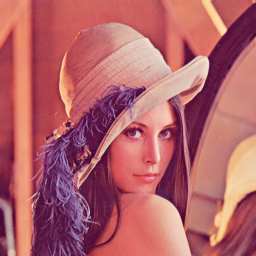
\includegraphics[width=\textwidth]{linear-1.png}
\end{figure}
\end{column}
\begin{column}{.3\textwidth}
\begin{figure}
\centering
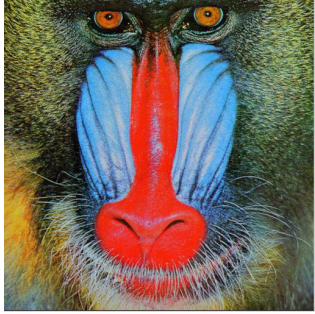
\includegraphics[width=\textwidth]{linear-3.png}
\end{figure}
\end{column}
\begin{column}{.3\textwidth}
\begin{figure}
\centering
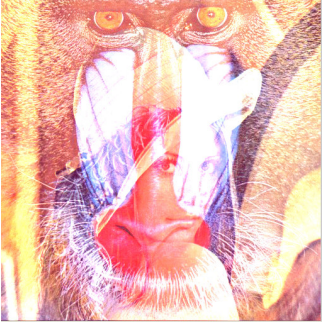
\includegraphics[width=\textwidth]{linear-4.png}
\end{figure}
\end{column}
\end{columns}
\end{frame}

%----------------------------------------------------------------------------------------

\begin{frame}
\begin{itemize}
\item Non-linear example; the Max operator.
\item Another example: Absolute image differencing:
\end{itemize}
\begin{columns}
\begin{column}{.3\textwidth}
\begin{figure}
\centering
\includegraphics[width=\textwidth]{linear-1.png}
\end{figure}
\end{column}
\begin{column}{.3\textwidth}
\begin{figure}
\centering
\includegraphics[width=\textwidth]{linear-3.png}
\end{figure}
\end{column}
\begin{column}{.3\textwidth}
\begin{figure}
\centering
\includegraphics[width=\textwidth]{linear-5.png}
\end{figure}
\end{column}
\end{columns}
\end{frame}


%----------------------------------------------------------------------------------------

\begin{frame}
\begin{itemize}
\item linear operations are important due to their theoretical and practical results applicable to image processing.
\item Nonlinear systems are not nearly as well understood, so their scope of application is more limited.
\end{itemize}
\end{frame}

%----------------------------------------------------------------------------------------

\subsection{Arithmetic operations}

%----------------------------------------------------------------------------------------

\begin{frame}
\begin{itemize}
\item The arithmetic operations ($+,-,\times, \div$) are performed pixelwise in array operations, between images of the same size.
\end{itemize}
Example of noise reduction using average. Assume:
\begin{enumerate}
\item An image $f(x,y)$ corrupted by noise:
\begin{equation}
g(x,y) = f(x,y) + \eta(x,y).
\end{equation}
\item The noise is uncorrelated between image acquisitions.
\item The noise has zero mean value.
\end{enumerate}
\end{frame}

%----------------------------------------------------------------------------------------

%\begin{frame}
%Important applications of image averaging for noise reduction:
%\begin{itemize}
%\item Astronomy. Uncorrelated and zero-averaged noise.
%\end{itemize}
%\begin{figure}
%\centering
%\includegraphics[width=.8\textwidth]{averaging.png}
%\end{figure}
%\footnote{galaxy pair NGC
%3314, taken by NASA’s
%Hubble Space Telescope.}
%\end{frame}

%----------------------------------------------------------------------------------------

\begin{frame}
Example of image subtraction application.
\begin{itemize}
\item Subtract images containing differences or movement.
\item The subtraction operation highlights differences.
\end{itemize}
\begin{columns}
\begin{column}{.5\textwidth}
\begin{figure}
\centering
\includegraphics[width=\textwidth]{subtraction-1.png}
\end{figure}
\end{column}
\begin{column}{.5\textwidth}
\begin{figure}
\centering
\includegraphics[width=\textwidth]{subtraction-2.png}
\end{figure}
\end{column}
\end{columns}
\end{frame}

%----------------------------------------------------------------------------------------

\begin{frame}
Another example:
\begin{figure}
\centering
\includegraphics[width=.8\textwidth]{head-contrast.png}
\end{figure}
\end{frame}

%----------------------------------------------------------------------------------------

\begin{frame}
\begin{block}{Attention!}
The image resulting form arithmetic operations should (often) be scaled to $[0,255]$!
\end{block}
\end{frame}

%----------------------------------------------------------------------------------------

\subsection{Set and logical operations}

%----------------------------------------------------------------------------------------

\begin{frame}
Basic set operations:
\begin{figure}
\centering
\includegraphics[width=.7\textwidth]{sets-1.png}
\end{figure}
\end{frame}

%----------------------------------------------------------------------------------------

\begin{frame}
Consider set $A$ formed of triplets $(x,y,z)$, where
\begin{itemize}
\item $x, y$ are spatial coordinates.
\item $z$ is intensity.
\end{itemize}
The \textit{complement} of $A$ is defined as
\[
A^{c}={(x,y,K-z)|(x,y,z)\in A},
\]
where
\[
K=2^{k}-1.
\]
e. g., $K = 255$ for 8 bits.
\end{frame}

%----------------------------------------------------------------------------------------

\begin{frame}
\begin{figure}
\centering
\includegraphics[width=.7\textwidth]{skeletons-1.png}
\end{figure}
\end{frame}

%----------------------------------------------------------------------------------------

\begin{frame}
The union of two gray-scale sets $A$ and $B$ may be defined as the set
\begin{equation}
A\cup B = \left \{ \max_z (a,b)| a\in A, b\in B \right \}
\end{equation}
\begin{figure}
\centering
\includegraphics[width=.9\textwidth]{skeletons-2.png}\footnote{$B=3\times \mu_{A}$}
\end{figure}
\end{frame}

%----------------------------------------------------------------------------------------

\begin{frame}
Logical operators.
\begin{figure}
\centering
\includegraphics[width=.4\textwidth]{logicalOperators.png}
\end{figure}
\end{frame}

%----------------------------------------------------------------------------------------

\subsection{Spatial operations}

%----------------------------------------------------------------------------------------

\begin{frame}
Spatial operations are performed directly on the pixels of a given image. The operations can be:
\begin{itemize}
\item Single-pixel.
\item Neighborhood.
\item Geometric spatial.
\end{itemize}
\end{frame}

%----------------------------------------------------------------------------------------

\begin{frame}
\frametitle{Single pixel operations}
\begin{itemize}
\item Alter the value of the pixels based on their intensities.
\end{itemize}
\begin{equation}
s = T(z).
\end{equation}
\begin{figure}
\centering
\includegraphics[width=.5\textwidth]{intensityTransformation.png}
\end{figure}
\end{frame}

%----------------------------------------------------------------------------------------

\begin{frame}
\frametitle{Neighborhood operations}
\begin{itemize}
\item Each pixel on the output image depends on the neighborhood of the corresponding (same position) pixel in the input image.
\end{itemize}
Example: Local averaging.
\begin{equation}
g(x,y) = \dfrac{1}{mn}\sum_{(x,y)\in S_{xy}}f(r,c).
\end{equation}
\begin{figure}
\centering
\includegraphics[width=.6\textwidth]{neighborhoodProcessing-1.png}
\end{figure}
\end{frame}

%----------------------------------------------------------------------------------------

\begin{frame}
The net effect is to perform local blurring in the original image.
\begin{figure}
\centering
\includegraphics[width=.7\textwidth]{neighborhoodProcessing-2.png}
\end{figure}
\end{frame}

%----------------------------------------------------------------------------------------

\begin{frame}
Median filter:
\begin{itemize}
\item Order the neighboring pixels in ascending order and sets the output to the median value.
\end{itemize}
\begin{figure}
\centering
\includegraphics[width=.7\textwidth]{median-1.png}
\end{figure}
\begin{itemize}
\item Good for filtering high valued noises:
\begin{figure}
\centering
\includegraphics[width=.5\textwidth]{median-2.png}
\end{figure}
\end{itemize}
\end{frame}

%----------------------------------------------------------------------------------------

\begin{frame}
\frametitle{Geometric spatial operations}
\begin{itemize}
\item Change the relation between pixel positions.
\item Two steps:
\begin{itemize}
\item Spatial transformation.
\begin{equation}
(x,y) = T\left \{ (u,v) \right \}
\end{equation}
\begin{itemize}
\item This process often creates pixels nonexistent in the original image, leading to the necessity of
\end{itemize}
\item Interpolation:
\begin{itemize}
\item Replication (nearest-neighbor), bi-linear, $\sin(x)/x$, etc$\ldots$.
\end{itemize}
\end{itemize}
\end{itemize}
\end{frame}

%----------------------------------------------------------------------------------------

\begin{frame}
A general form that can \textit{scale}, \textit{translate}, \textit{rotate} or \textit{sheer} a set of coordinate points is the \textit{Affine} transform:
\begin{figure}
\centering
\includegraphics[width=.7\textwidth]{affineTransform.png}
\end{figure}
\end{frame}

%----------------------------------------------------------------------------------------

\begin{frame}
\begin{figure}
\centering
\includegraphics[width=\textwidth]{affineTransform-1.png}
\end{figure}
\end{frame}

%----------------------------------------------------------------------------------------

\begin{frame}
\begin{figure}
\centering
\includegraphics[width=\textwidth]{affineTransform-2.png}
\end{figure}
\end{frame}

%----------------------------------------------------------------------------------------

\begin{frame}
\begin{figure}
\centering
\includegraphics[width=\textwidth]{rotation.png}
\end{figure}
\end{frame}

%----------------------------------------------------------------------------------------

\begin{frame}
\frametitle{Image registration}
Input and output images are given and the transformation must be estimated.
\begin{itemize}
\item Examples: Change detection in satellite images.
\item Before comparison, images must be corrected to fix acquisition misalignment.
\item \textit{Ground Control Points} (GCP) are often used in aerial photography.
\item Small metallic objects embedded in the sensor produce \textit{known} points that can also be used as reference.
\item Image descriptors (SIFT, SURF, etc).
\end{itemize}
\end{frame}

%----------------------------------------------------------------------------------------

\begin{frame}
\begin{figure}
\centering
\includegraphics[width=\textwidth]{registration-1.png}
\end{figure}
\end{frame}

%----------------------------------------------------------------------------------------

\begin{frame}
\begin{figure}
\centering
\includegraphics[width=\textwidth]{registration-2.png}
\end{figure}
\end{frame}

%----------------------------------------------------------------------------------------

\begin{frame}
\begin{figure}
\centering
\includegraphics[width=.7\textwidth]{ocv-stitching.png}
\end{figure}
\end{frame}

%----------------------------------------------------------------------------------------
%
%\subsection{Vector and matrix operations}
%
%%----------------------------------------------------------------------------------------
%
%\begin{frame}
%
%\end{frame}

%----------------------------------------------------------------------------------------

\subsection{Image transforms}

%----------------------------------------------------------------------------------------

\begin{frame}
\begin{itemize}
\item So far, processing was presented only in the spatial domain (directly upon pixels).
\item Another tools arise when transforming images into other domains, such as frequency, as illustrated below.
\end{itemize}
\begin{equation}
T(u,v) = \sum_{x=0}^{M-1}\sum_{y=0}^{N-1}f(x,y) r(x,y,u,v).
\end{equation}
where:
\begin{itemize}
\item $f(x,y)$ - input image.
\item $r(x,y,u,v)$ - forward transformation kernel.
\item $x, y$ - spatial variables.
\item $M, N$ row and column dimensions of $f(x,y)$.
\item $u=0,\ldots,M-1$ and $v=0,\ldots,N-1$ form the transformed coordinate system.
\end{itemize}
\end{frame}

%----------------------------------------------------------------------------------------

\begin{frame}
Given $T(u,v)$, $f(x,y)$ can be recovered from the inverse transform:
\begin{equation}
f(x,y) = \sum_{u=0}^{M-1}\sum_{v=0}^{N-1}T(u,v) s(x,y,u,v).
\end{equation}
where:
\begin{itemize}
\item $f(x,y)$ - recovered image.
\item $s(x,y,u,v)$ - backward transformation kernel.
\item $x, y$ - spatial variables.
\item $M, N$ row and column dimensions of $f(x,y)$.
\item $x=0,\ldots,M-1$ and $y=0,\ldots,N-1$ form the spatial coordinate system.
\end{itemize}
\end{frame}

%----------------------------------------------------------------------------------------

\begin{frame}
\begin{figure}
\centering
\includegraphics[width=\textwidth]{imgTransform.png}
\end{figure}
\begin{figure}
\centering
\includegraphics[width=.6\textwidth]{moonFFT.png}
\end{figure}
\end{frame}

%----------------------------------------------------------------------------------------

\subsection{Probabilistic methods}

%----------------------------------------------------------------------------------------

\begin{frame}
Intensity values in an image can be considered random quantities:
\begin{itemize}
\item Let $z_{i}, i=0,\ldots,L-1$, denote the values of all possible intensities in an $M\times N$ digital image.
\item The probability $p(z_{k})$, of intensity level $z_{k}$ occurring is
\begin{equation}
p(z_{k}) = \dfrac{n_{k}}{MN},
\end{equation}
where $n_{k}$ is the number of occurrences of $z_{k}$ and $MN$ is the total number of pixels.
\item Note that $\sum_{k=0}^{L-1}p(z_{k}) = 1$.
\end{itemize}
\end{frame}

%----------------------------------------------------------------------------------------

\begin{frame}
Given $p(z_{k})$, other image characteristics can be obtained, such as
\begin{itemize}
\item Image mean \[m=\sum_{k=0}^{L-1}z_{k}p(z_{k}).\]
\item Variance \[\sigma^{2}=\sum_{k=0}^{L-1}\left ( z_{k} - m \right )^{2} p(z_{k}).\]
\item \textit{n}th moment of random variable $z$ about the mean \[\mu_{n}(z) = \sum_{k=0}^{L-1}\left ( z_{k} - m \right )^{n} p(z_{k}).\]
\end{itemize}
\end{frame}

%----------------------------------------------------------------------------------------

\begin{frame}
Notice that
\begin{itemize}
\item $\mu_{0}(z) = 1$.
\item $\mu_{1}(z) = 0$.
\item $\mu_{2}(z) = \sigma^{2}$.
\end{itemize}
\end{frame}

%----------------------------------------------------------------------------------------

\begin{frame}
\begin{itemize}
\item The mean and variance are more easily associated with the intensity distribution on an image.
\item Higher moments, however, are more subtle.
\item Example, $\mu_{3}$:
\begin{itemize}
\item $\mu_{3} > 0$, distribution skewed to the right.
\item $\mu_{3} = 0$, distribution symmetrically skewed.
\item $\mu_{3} < 0$, distribution skewed to the left.
\end{itemize}
\end{itemize}
\end{frame}

%----------------------------------------------------------------------------------------

\begin{frame}
Example of an image with low, medium and high contrast with, respectively, 14, 32 and 50 standard deviations.
\begin{figure}
\centering
\includegraphics[width=\textwidth]{einsteinContrast.png}
\end{figure}
\end{frame}

%----------------------------------------------------------------------------------------

\begin{frame}
Probabilistic methods are broadly used in image processing:
\begin{itemize}
\item Intensity transformations.
\item Restoration.
\item Segmentation.
\item Texture description.
\item Object recognition.
\end{itemize}
\end{frame}

%----------------------------------------------------------------------------------------

\end{document}


%----------------------------------------------------------------------------------------
